\documentclass[letterpaper,12pt,oneside]{article}\usepackage[]{graphicx}\usepackage[]{color}
%% maxwidth is the original width if it is less than linewidth
%% otherwise use linewidth (to make sure the graphics do not exceed the margin)
\makeatletter
\def\maxwidth{ %
  \ifdim\Gin@nat@width>\linewidth
    \linewidth
  \else
    \Gin@nat@width
  \fi
}
\makeatother

\definecolor{fgcolor}{rgb}{0.345, 0.345, 0.345}
\newcommand{\hlnum}[1]{\textcolor[rgb]{0.686,0.059,0.569}{#1}}%
\newcommand{\hlstr}[1]{\textcolor[rgb]{0.192,0.494,0.8}{#1}}%
\newcommand{\hlcom}[1]{\textcolor[rgb]{0.678,0.584,0.686}{\textit{#1}}}%
\newcommand{\hlopt}[1]{\textcolor[rgb]{0,0,0}{#1}}%
\newcommand{\hlstd}[1]{\textcolor[rgb]{0.345,0.345,0.345}{#1}}%
\newcommand{\hlkwa}[1]{\textcolor[rgb]{0.161,0.373,0.58}{\textbf{#1}}}%
\newcommand{\hlkwb}[1]{\textcolor[rgb]{0.69,0.353,0.396}{#1}}%
\newcommand{\hlkwc}[1]{\textcolor[rgb]{0.333,0.667,0.333}{#1}}%
\newcommand{\hlkwd}[1]{\textcolor[rgb]{0.737,0.353,0.396}{\textbf{#1}}}%

\usepackage{framed}
\makeatletter
\newenvironment{kframe}{%
 \def\at@end@of@kframe{}%
 \ifinner\ifhmode%
  \def\at@end@of@kframe{\end{minipage}}%
  \begin{minipage}{\columnwidth}%
 \fi\fi%
 \def\FrameCommand##1{\hskip\@totalleftmargin \hskip-\fboxsep
 \colorbox{shadecolor}{##1}\hskip-\fboxsep
     % There is no \\@totalrightmargin, so:
     \hskip-\linewidth \hskip-\@totalleftmargin \hskip\columnwidth}%
 \MakeFramed {\advance\hsize-\width
   \@totalleftmargin\z@ \linewidth\hsize
   \@setminipage}}%
 {\par\unskip\endMakeFramed%
 \at@end@of@kframe}
\makeatother

\definecolor{shadecolor}{rgb}{.97, .97, .97}
\definecolor{messagecolor}{rgb}{0, 0, 0}
\definecolor{warningcolor}{rgb}{1, 0, 1}
\definecolor{errorcolor}{rgb}{1, 0, 0}
\newenvironment{knitrout}{}{} % an empty environment to be redefined in TeX

\usepackage{alltt}
\usepackage[paperwidth=8.5in,paperheight=11in,top=1in,bottom=1in,left=1in,right=1in]{geometry}
\usepackage{setspace}
\usepackage[colorlinks=true,allcolors=Blue]{hyperref}
\usepackage[usenames,dvipsnames]{xcolor}
\usepackage{indentfirst}
\usepackage{titlesec}
\usepackage{multirow}
\usepackage{booktabs}
\usepackage{graphicx}
\usepackage{verbatim}
\usepackage{rotating}
\usepackage{tabularx}
\usepackage{outlines}
\usepackage{lineno}
\usepackage{array}
\usepackage{times}
\usepackage{cleveref}
\usepackage{acronym}
\usepackage[position=t]{subfig}
\usepackage{paralist}
\usepackage[noae]{Sweave}
\usepackage{natbib}
\usepackage{array}
\usepackage{pdflscape}
\usepackage{bm}
\usepackage{showlabels}
\bibpunct{(}{)}{,}{a}{}{,}

% page margins and section title formatting
\linespread{2}
\setlength{\footskip}{0.5in}
\titleformat*{\section}{\Large\bf\em}
\titleformat*{\subsection}{\singlespace\large\bf}
\titleformat*{\subsubsection}{\singlespace\normalsize\bf\em}
\titlespacing{\section}{0in}{0in}{0in}
\titlespacing{\subsection}{0in}{0in}{0in}
\titlespacing{\subsubsection}{0in}{0in}{0in}

% cleveref options
\crefname{table}{Table}{Tables}
\crefname{figure}{Fig.}{Figs.}
\renewcommand{\figurename}{Fig.}

% aliased citations
\defcitealias{HagyIR}{Hagy, In review}

%acronyms
\acrodef{DEM}{Digital Elevation Model}
\acrodef{EPA}{Environmental Protection Agency}
\acrodef{doc}[DoC]{depth of colonization}
\acrodef{GIS}{Geographic Information System}
\acrodef{NOAA}{National Oceanic and Atmospheric Administration}

%knitr options


\IfFileExists{upquote.sty}{\usepackage{upquote}}{}
\begin{document}

\raggedbottom
\linenumbers
\raggedright
\urlstyle{same}
\setlength{\parindent}{0.5in}
\renewcommand\refname{References \vspace{12pt}}

\begin{singlespace}
\title{{\bf {\Large Spatially-referenced estimates of seagrass depth of colonization}}}
\author{
  {\bf {\normalsize Marcus W. Beck$^1$, James D. Hagy III$^2$}}
  \\\\{\textit {\normalsize $^1$ORISE Research Participation Program}}
  \\{\textit {\normalsize USEPA National Health and Environmental Effects Research Laboratory}}
  \\{\textit {\normalsize Gulf Ecology Division, 1 Sabine Island Drive, Gulf Breeze, FL 32561}}
	\\{\textit {\normalsize Phone: 850-934-2480, Fax: 850-934-2401, Email: \href{mailto:beck.marcus@epa.gov}{beck.marcus@epa.gov}}}
  \\\\{\textit {\normalsize $^2$USEPA National Health and Environmental Effects Research Laboratory}}
	\\{\textit {\normalsize Gulf Ecology Division, 1 Sabine Island Drive, Gulf Breeze, FL 32561}}
	\\{\textit {\normalsize Phone: 850-934-2455, Fax: 850-934-2401, Email: \href{mailto:hagy.jim@epa.gov}{hagy.jim@epa.gov}}}
	}
\date{}
\maketitle
\end{singlespace}
\clearpage

\section{Introduction}

Issues related to excessive nutrient pollution have motivated a substantial body of research to understand and address impacts on coastal waters.  Eutrophication, defined as an increase in the rate of supply of organic matter to an ecosystem \citep{Nixon95}, is primarily caused by anthropegenic inputs of limiting nutrients that exceed background concentrations of receiving waters.  Adverse impacts on aquatic resources are well-documented and have included increased occurrence in the frequency and severity of harmfal algal blooms \citep{Cloern96}, reduction of dissolved oxygen necessary to support heterotrophic organisms \citep{Justic87,Diaz08}, and loss of ecosystem functioning through food web simplification \citep{Tewfik07}. Although management activities have been successful in mitigating or reversing eutrophication impacts (e.g., \citealt{Greening06}), the evaluation of response endpoints remains an important topic given that ecosystem changes in relation to different nutrient regimes are not fully understood nor anticipated \citep{Duarte09}.  The most appropriate indicators of ecosystem response may be those that exhibit clear biological linkages with water quality changes, such that the potential effects of management actions can be unambiguously characterized through known cause and effect pathways.  Critical management decisions may be forced by tentative assessments, political motivations, or qualitative criteria in the absence of empirical methods to identify adequate indicators of ecosytem response \citep{Duarte09}.  

The ecosystem services provided by seagrasses as well as their sensitivity to water quality changes has contributed to the proliferation of their use as biological response endpoints for eutrophication.  Seagrasses are ecosystem engineers \citep{Jones94,Koch01} that serve a structural and functional role in altering aquatic habitat often through different feedback mechanisms with other ecosystem components.  For example, seagrass beds create habitat for juvenile fish and crabs by reducing wave action and stabilizing sediment \citep{williams01,Hughes09}.  Seagrasses also respond to changes in water clarity through direct physiological linkages with light availability.  In short, increased nutrient loading contributes to reductions in water clarity through increased algal concentrations, inhibiting the growth of seagrass through light limitation \citep{Duarte95}.  Empirical relationships between nutrient loading, water clarity, light requirements, and the maximum depth of seagrass colonization have been identified \citep{Duarte91,Kenworthy96,Choice14}, such that quantitative standards have been developed to maintain light regimes sufficient for seagrass growth targets \citep{Steward05}.  The converse has also been used such that seagrass depth limits have formed the basis of quantititative criteria for nutrient load targets \citep{Janicki96}.  Contrasted with numeric standards for nutrients and phytoplankon, seagrass-based critiera may be more useful for standards development given that seagrasses are integrative of system-wide conditions over time and less variable with changes in nutrient regimes \citep{Duarte95}.  

The development of numeric criteria and standards for coastal waters has been a management priority within the United States \citep{USEPA98} and internationally \citep{WFD00}.  Numerous agencies and management programs have developed a variety of techniques for estimating seagrass depth limits as a basis for establishing numeric criteria, either as restoration targets or for identifying critical load limits.  Such efforts have been useful for site-specific approaches where the analysis needs are driven by the particular management or research context \citep[e.g.,][]{Iverson86,Hale04}. However, a lack of standardization among methods has prevented broad-scale comparisons between regions and has even contributed to discrepancies between measures of depth limits based on chosen technique.  For example, seagrass depth limits based on in situ techniques can vary with the sampling device \citep{Spears09}.  Despite the availability of data, techniques for estimating seagrass depth of colonization using remotely sensed data have not been extensively developed.  Such techniques have the potential to facilitate broad-scale comparisons between regions given the spatial coverage and annual availability of many products.  For example, recent analyses by \citetalias{HagyIR} have shown that standardized techniques from seagrass coverage maps and bathymetric data can be used to compare growth patterns over time among different coastal regions of Florida.  Such methods show promise, although further development to improve the spatial resolution of are needed.  Specifically, methods for estimating seagrass depth limits should be reproducible for broad-scale comparisons, while also maintaining flexibility for site-specific estimates depending on management needs.

Reproducible and empirical approaches can be developed to provide more consistent estimates of seagrass depth limits for restoration targets or criteria development. This analysis describes a method for estimating seagrass depth of colonization using information-rich datasets to create a spatially explicit and repeatable estimate.  In particular, methods described in \citetalias{HagyIR} are improved upon by creating a flexible and repeatable technique for estimating seagrass depth limits from coverage maps and bathymetric data. The specific objectives are to \begin{inparaenum}[1\upshape)]
\item describe the method for estimating seagrass depth limits within a relevant spatial context, 
\item apply the technique to four distinct regions of Florida to illustrate improved clarity of description, and
\item develop a spatially coherent relationship between depth limits and water clarity for the case studies.  
\end{inparaenum}
Overall, these methods are expected to inform the development of water quality criteria based on empirical relationships of seagrass depth limits with water clarity over time.  The method is applied to data from Florida although the technique is transferable to other regions with comparable data. 

\section{Methods}

Development of a spatially-referenced approach to estimate seagrass \ac{doc} relied extensively on data and partially on methods described in \citetalias{HagyIR}.  The following is a summary of locations and data sources, methods in \citetalias{HagyIR}, methods and rationale developed to incorporate spatial information in seagrass \ac{doc}, and evaluation of the approach including relationships with water clarity.   

\subsection{Locations and data sources}

Four unique locations were chosen for the analysis: Choctowatchee Bay (Panhandle), Big Bend region (northeast Gulf of Mexico), Tampa Bay (central Gulf Coast of Florida), and Indian River Lagoon (east coast) ().  These locations were chosen to represent the different geographic regions in the state, in addition to data availability and observed gradients in water clarity that likely contributed to hetereogeneity in seagrass growth patterns.  For example, the Big Bend region was chosen to an outflow of the Steinhatchee River where higher concentrations of dissolved organic matter are observed.  Seagrasses near the outflow were observed to grow at shallower depths as compared to locations far from the river source.  Coastal regions and estuaries in Florida are divided into individual spatial units based on a segmentation scheme developed by US \ac{EPA} for the development of numeric nutrient criteria.  One segment from each geographic location was used for the analysis to evaluate estimates of seagrass \ac{doc}.  The segments included numbers 0303 (Choctowatchee Bay), 0820 (Big Bend region), 0902 (Tampa Bay), and 1502 (Indian River Lagoon), where the first two digits indicate the estuary and the last two digits indicate the segment within the estuary. 

Data used to estimate seagrass \ac{doc} included a suite of publically available \ac{GIS} products.  At the most generic level, spatially-referenced information describing seagrass aerial coverage combined with co-located bathymetric depth information were used to estimate \ac{doc}.  These data products are available in coastal regions of Florida through the US Geological Survey, Florida Department of Environmental Protection, and watershed management districts.  Data are generally more available in larger estuaries that are of specific management concern, e.g., Tampa Bay, Indian River Lagoon.  For example, seagrass coverage data are available from 1950 (Tampa Bay) to present day (multiple estuaries), with more recent products available at annual or  biennial intervals.  Seagrass coverage maps are less frequent in areas with lower population densities (e.g., Big Bend region) or where seagrass is naturally absent (northeast Florida).  Seagrass maps were produced using photo-interpretations of aerial images to categorize coverage as absent, discontinuous (patchy), or continuous.  For this analysis, we considered seagrass coverage as being only present (continuous and patchy) or absent since the former did not represent unequivocal categories between regions. 

Seagrass coverage maps were combined with bathymetric depth layers to characterize location and depth of growth in each location.  Bathymetric depth layers for each location were obtained from the National Oceanic and Atmospheric Administration's (\acsu{NOAA}) National Geophysical Data Center as either \acp{DEM} or raw sounding data from hydroacoustic surveys.  Tampa Bay data provided by the Tampa Bay National Estuary Program are described in \citet{Tyler07}. Bathymetic data for the Indian River Lagoon were obtained from the St. John's Water Management District \citep{CPE97}.  \ac{NOAA} products were referenced to mean lower low water, whereas Tampa Bay data were referenced to the North American Vertical Datum of 1988 and the Indian River Lagoon data were referenced to mean sea level.  Depth layers were combined with seagrass coverage layers using standard union techniques of raster and vector layers in ArcMap 10.1 \citep{ESRI12}.  To reduce computation time, depth layers were first masked using a 1 km buffer of the seagrass coverage layer.  The final layer used for analysis was a point layer with attributes describing location (latitude, longitude, segment), depth (m), and seagrass (present, absent).  Additional details describing the data are available in \citetalias{HagyIR}.    

\subsection{Segment-based estimates of seagrass depth of colonization}

Methods in \citetalias{HagyIR} describe an approach for estimating seagrass \ac{doc} at individual coastal segments.  Specifically, the combined seagrass depth data described above are used to estimate maximum ($Z_{cMax}$) and median ($Z_{c50\%}$) seagrass \ac{doc}, where the maximum depth is defined as the deepest depth at which a ``significant'' coverage of seagrasses occured in a segment and the median depht is defined as the median depth occurring at the deep water edge. The seagrass depth points are grouped into bins and the proportion of points within each depth bin that contain seagrass are quantified.  Both seagrass \ac{doc} estimates are obtained from the plot of proportion of points occupied at each depth bin.  In general, the plot is characterized by a decreasing trend such that the proportion of occupied points by depth bin decreases and eventually flattens with increasing depth.  A regression is fit on this descending portion of the curve such that the intercept point on the x-axis is considered the maximum depth of colonization.  The median portion of this curve is considered the median depth of the deepwater edge of seagrass.   

Considerable spatial heterogeneity in the observed seagrass growth patterns suggests that a segment-wide estimate of seagrass \ac{doc} may be inappropriate, particularly for the examples in the current analysis. \Cref{fig:wbid_doc2} illustrates spatial variation in seagrass distribution  for a location in the Big Bend region of Florida.  Using methods in \citetalias{HagyIR}, the estimate for median seagrass \ac{doc} for the segment is over- and under-estimated for different areas of the segment.  In particular, \ac{doc} is greatly over-estimated at the outflow of the Steinhatchee where high concentrations of dissolved organic matter naturally limit seagrass growth.  This example suggests that estimates of \ac{doc} may be needed at finer spatial scales to provide a more robust determination of restoration targets and nutrient criteria.

\subsection{Estimating seagrass depth of colonization using spatial information}

The approach used to estimate seagrass \ac{doc} with spatial information has a similar theoretical foundation as the original, although several key differences should be noted.  In general, seagrass \ac{doc} estimates are based on empirical measures of the frequency occurrence of seagrass by increasing depth.  The first difference is that the maximum \ac{doc} is estimated from a logistic growth curve fit through the data, as compared to a simple linear regression in the previous example.  Second, a third measure describing the depth at which seagrass were most commonly located, as compared to maximum depth of growth, was defined using these methods.  The third and most important difference is that the estimates are specific to discrete locations, using either a grid of points or as a single location of interest. Methods and implications of these differences are described below.                                   

The spatially-referenced approach for estimating \ac{doc} begins by creating a grid of evenly-spaced points within the segment.  The same process for estimating \ac{doc} is used for each point.  Alternatively, a single location of interest can be chosen rather than a grid-based design with multiple estimates.  Seagrass depth data that occur within a set radius from each grid point are selected (\cref{fig:buff_ex}).  An estimate of seagrass \ac{doc} for each point in the grid is obtained using the sampled seagrass depth points.  The seagrass \ac{doc} estimate for each grid location is quantified from a plot of the proportion of bathymetric soundings that contain seagrass at each depth bin (\cref{fig:est_ex1}).  A radius around a grid point for sampling seagrass depth points that is sufficient to quantify depth of colonization typically has a plot similar to \cref{fig:est_ex1}.  The proportion of points that are occupied by seagrass should decrease continuously with increasing depth.  

A decreasing logistic growth curve is fit to the sampled seagrass depth points for the grid location to create a monotonic and asymptotic function.  This curve is fit using non-linear regression to characterize the reduction in points occupied by seagrass as a function of depth.  The logistic growth curve is fit by minimizing the residual sums-of-squares with the Gauss-Newton algorithm \citep{Bates92} and user-supplied starting parameters that are an approximate estimate of the curve characteristics.  The model has the following form:
\begin{equation}
 Proportion = \frac{\alpha}{1 + \mathrm{e}^{{\left(\beta - Depth\right)/\gamma}}}
\end{equation}
where the proportion of points occupied by seagrass at each depth is defined by a logistic curve with an asymptote $\alpha$, a midpoint inflection $\beta$, and a scale parameter $\gamma$.  Starting values $\alpha$, $\beta$, and $\gamma$ were estimated empirically from the observed data.  

Finally, a simple linear curve is fit through the inflection point ($\beta$) of the logistic curve to estimate depth of colonization (\cref{fig:est_ex3}).  The inflection point is the depth at which seagrass are decreasing at a maximum rate and is used as the slope of the linear curve.  Three measures are obtained from the linear curve. The maximum depth of seagrass colonization, $DOC_{max}$, is the x-axis intercept of the linear curve.  The depth of maximum seagrass occupancy, $SG_{max}$ is the location where the linear curve intercepts the asymptote of the logistic growth curve.  The median depth of seagrass colonization, $DOC_{med}$, is the depth halfway between $SG_{max}$ and $DOC_{max}$.  $DOC_{med}$ was typically but not always the inflection point of the logistic growth curve.  The estimation process is repated for each point in the grid.   

Estimates for each of the three \ac{doc} measures are obtained only if specific criteria are met.  These criteria were implemented as a safety measure that ensures a sufficient amount and appropriate quality of data are used.  First, estimates are provided only if a sufficient number of seagrass depth points are present within the radius of the grid point to estimate a logistic growth curve.  This criteria applies to the sample size as well as the number of points with seagrass in the sample.  That is, the curve cannot be estimated for small samples or if an insufficient number of points contain seagrass regardless of sample size.  Second, estimates are provided only if an inflection point is present on the logistic curve within the range of the sampled depth data.  This criteria may apply under two scenarios where the curve is estimated but a trend is not adequately described by the sampled data.  That is, a curve may be estimated that describes only the initial decrease in points occupied as a function of depth but the observed points do not occur at depths deeper than the predicted inflection point.  The opposite scenario may occur where a curve is estimated but only the deeper locations beyond the inflection point are present in the sample.  Finally, the estimate for $SG_{max}$ is set to zero if the linear curve through the inflection point intercepts the asympote at x-axis values less than zero.  The estimate for $DOC_{med}$ is also shifted to the depth value halfway between $SG_{max}$ and $DOC_{max}$.  

All estimates were obtained using custom-made functions in program R that were based on the \texttt{nls} and \texttt{SSlogis} functions to fit a nonlinear least squares using a self-starting logistic growth model \citep{Bates92,RDCT14}.  All seagrass depth shapefiles were imported and processed in R using functions in the \texttt{rgeos} and \texttt{sp} packages \citep{Bivand08,Bivand14}.  

\subsection{Comparison with segment-based approach and sensitivity analysis}

Spatially-referenced estimates for seagrass \ac{doc} were obtained for each of the four segments described above.  Segment-wide estimates obtained using methods in \citetalias{HagyIR} were used as a basis of comparison such that departures from these values were evidence of spatial heterogeneity in seagrass growth patterns within each segment.  A sampling grid of locations for estimating each of the three depth values in \cref{fig:est_ex} was created for each segment.  This grid is a set of evenly spaced points with a random starting location for the first point.  The grid is masked by the segment boundaries to remove locations that did not occur on the water.  Initial spacing between sample points was chosen arbitrarily as 0.02 decimal degrees, which is approximately 2 km at 30 degrees N latitude.  Similarly, the sampling radius around each sampling location in the grid was chosen as 0.06 decimal degrees, or approximately 6 km.  

Three factors influence the estimates at each sampling point, as well as the ability compare values between points.  First, the starting location of the first point of the sampling grid is chosen arbitrarily such that a unique grid is obtained comparisons of within-segment estimates may vary slightly given the starting location.  Second, the spacing between sampling points affects the degree of collinearity between estimates that are near each other.  For a set sampling radius around each point, estimates will be less correlated at larger spacing between sampling points, whereas the converse is true for smaller spacing.  Third and most important, the radius around each sampling point determines the number of seagrass depth points that are included in the estimate.  The chosen radius is considered an explicit area within which the estimate applies.  As before, increasing the radius around each sample point will increase the collinearity between estimates at adjacent points for a set grid spacing.  Collinearity between sample points based on the sampling scheme is not inherently problematic provided the results are interpreted in the context of the question of interest.  For example, small spacing and large sampling radii will create very similar estimates between points.  This approach does not necessarily invalidate the estimate at each point, although comparisons between points become less valid as the estimates are not related to a unique sampling area for each location.  Similarly, a grid with large spacing and small radii facilitates comparison between points as each location represents a unique collection of samples, although each estimate is relevant for a small location with undescribed and potentially important variation in seagrass growth patterns between points.  

A systematic approach was used to evaluate validity of comparisons between sampling points given parameters that influence collinearity or spatial autocorrelation.  For the analysis, `validity' is considered relative uniqueness of estimates at each point in the context of grid spacing and sampling radius.  The effect of the random starting location of each grid was considered negligible for this analysis and set constant between analyses for comparison.  For each segment, unique combinations of grid spacing and sampling radii were used to estimate maximum seagrass \ac{doc}.  Spatial autocorrelation between all estimates was measured by semivariance 


\subsection{Developing a spatially coherent relationship of water clarity with depth of colonization}

\section{Results}

\section{Discussion}

% qualitative and quantitative advantages of the approach

%%%%%%
% refs
\clearpage
\begin{singlespace}
\bibliographystyle{apalike_mine}
\bibliography{ref_sgdepth}
\end{singlespace}
\clearpage

%%%%%%
% figures

% example of depth of col ests for wbid - big bend 820
\begin{figure}
\centerline{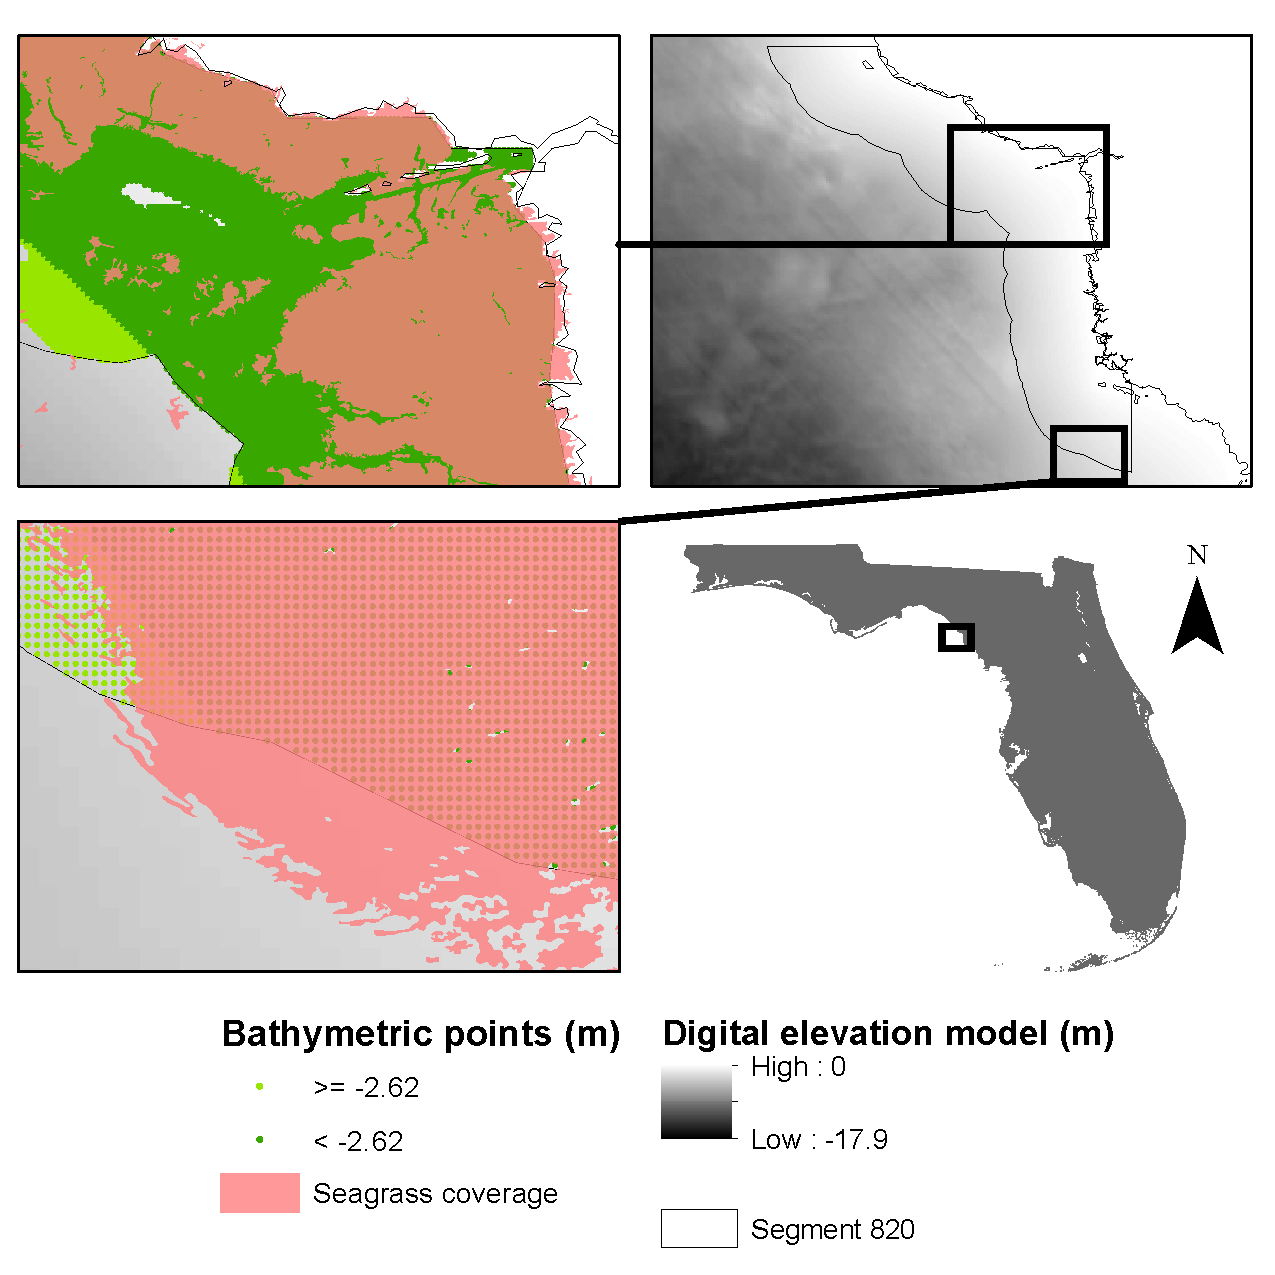
\includegraphics[width = \textwidth]{figs/wbid_doc2.pdf}}
\caption{Example of over- and under-estimates for seagrass depth of colonization for a segment in the Big Bend region, Florida.  The top-left figure indicates over-estimation and the bottom-left indicates under-estimation.  Bathymetric points are color-coded by the median depth of colonization estimate for continuous seagrass in the segment.}
\label{fig:wbid_doc2}
\end{figure}

% example of buffer points for depth of col


% example of buffer points for depth of col
\begin{figure}
\centering
\subfloat[][Seagrass depth points for the segment]{
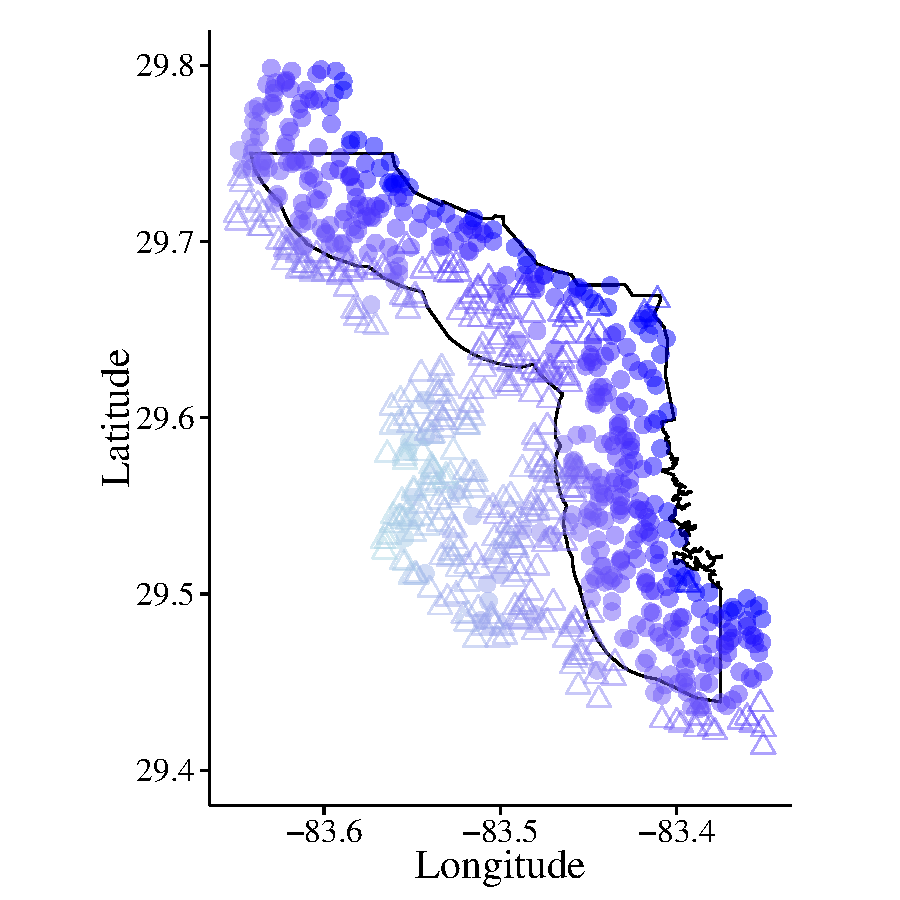
\includegraphics[width=0.5\textwidth]{figs/buff_ex1.pdf}
\label{fig:buff_ex1}
}
\subfloat[][Grid of locations and sample areas for estimates]{
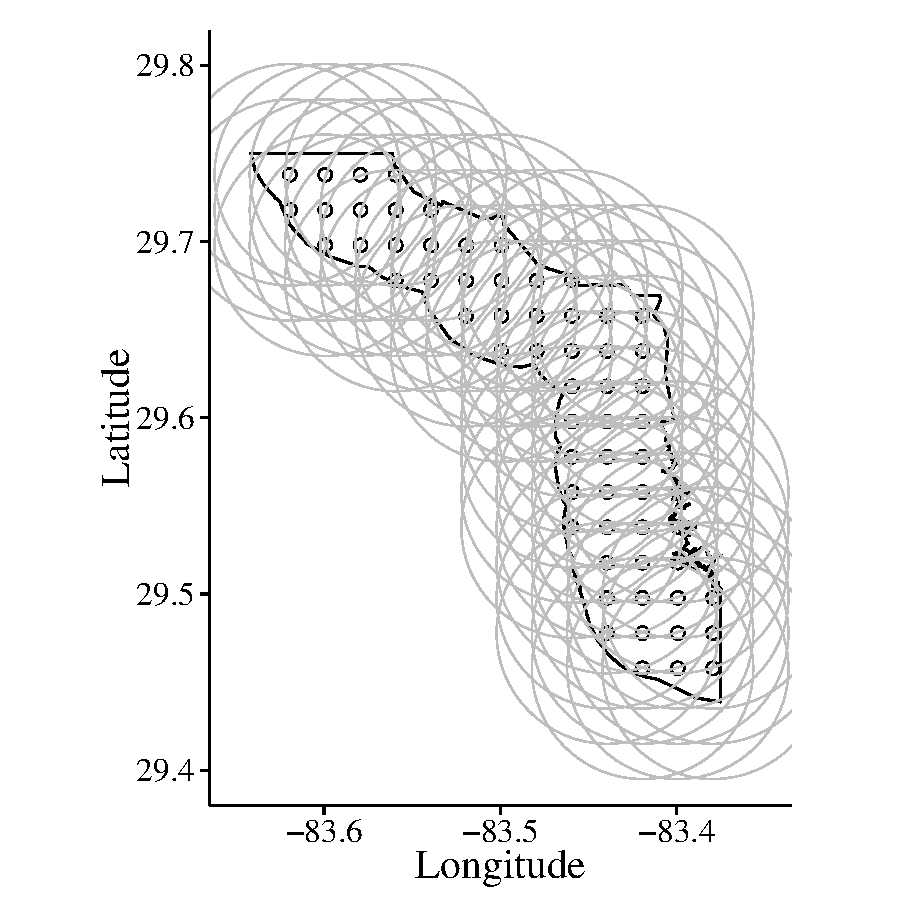
\includegraphics[width=0.5\textwidth]{figs/buff_ex2.pdf}
\label{fig:buff_ex2}
}

\subfloat[][Sampled observations for a test point]{
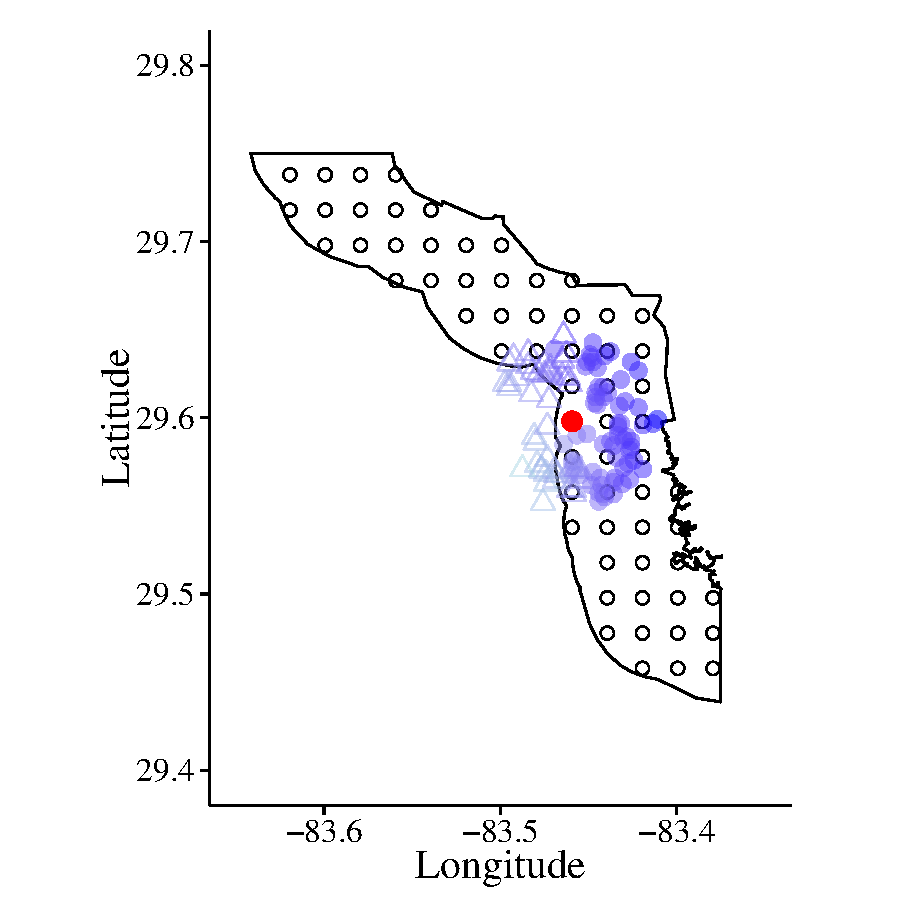
\includegraphics[width=0.5\textwidth]{figs/buff_ex3.pdf}
\label{fig:buff_ex3}
}
\subfloat{
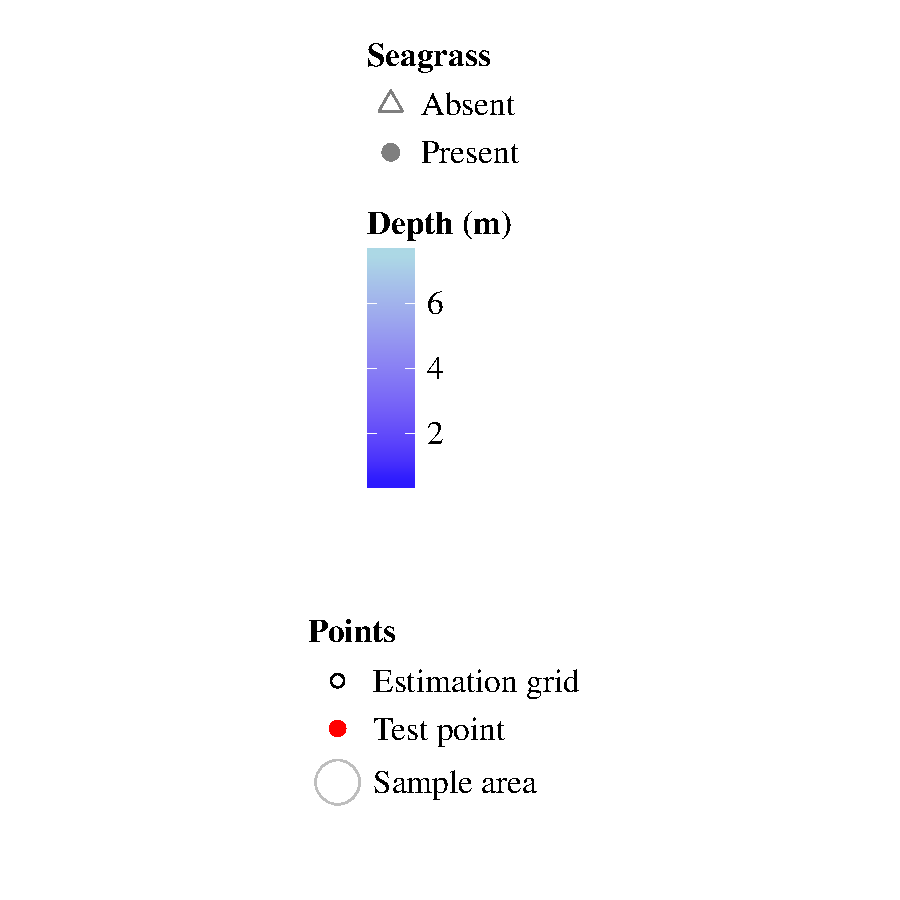
\includegraphics[width = 0.5\textwidth]{figs/buff_ex4.pdf}
}
\caption{Examples of data and grid locations for estimating seagrass depth of colonization for a region of the Big Bend, Florida.  \Cref{fig:buff_ex1} shows the seagrass depth points that are used for sampling, \cref{fig:buff_ex2} shows a grid of locations and sampling radii for estimating seagrass \ac{doc}, and \cref{fig:buff_ex3} shows an example of sampled seagrass depth points for a location.  Estimates in \cref{fig:est_ex} were obtained from the sampled location in \cref{fig:buff_ex3}.}
\label{fig:buff_ex}
\end{figure}

% example of estimating seagrass depth of colonization


% example of depth of col ests for wbid - big bend 820
\begin{figure}
\centering
\subfloat[][Proportion of points with seagrass by depth]{
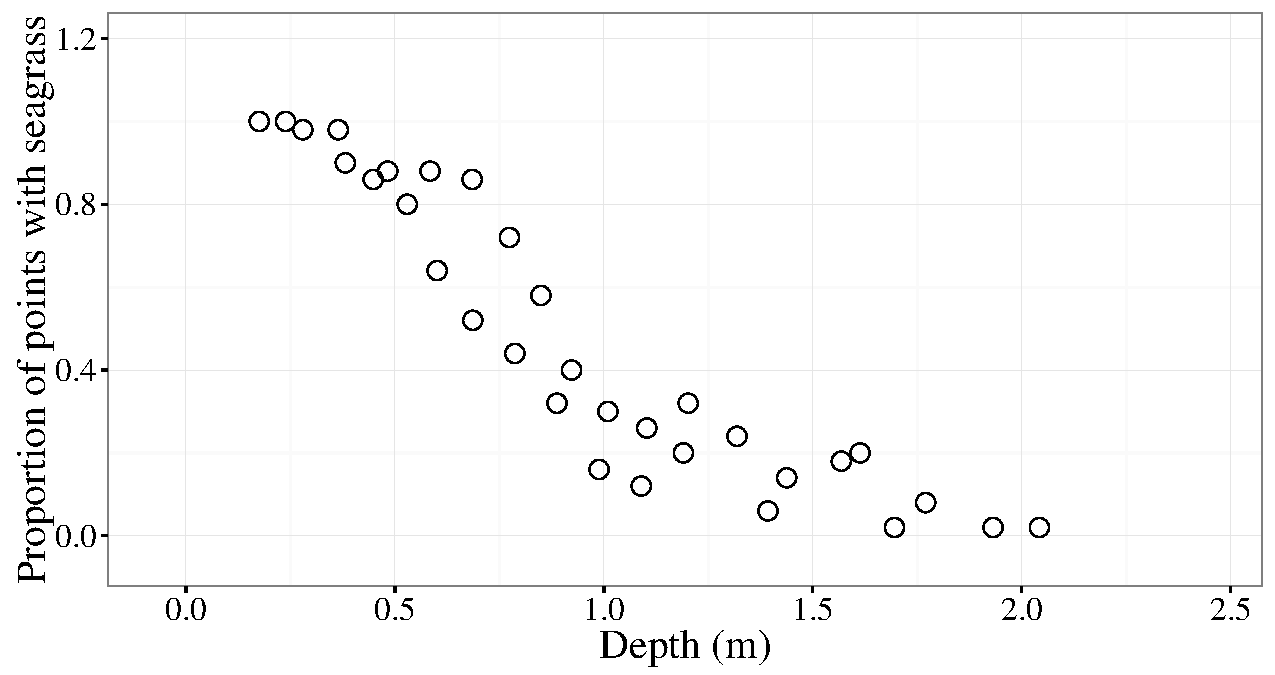
\includegraphics[page=1,width=0.5\textwidth]{figs/est_ex.pdf}
\label{fig:est_ex1}
}

\subfloat[][Logistic growth curve fit through points]{
\includegraphics[page=2,width=0.5\textwidth]{figs/est_ex.pdf}
\label{fig:est_ex2}
}

\subfloat[][Depth estimates]{
\includegraphics[page=3,width=0.5\textwidth]{figs/est_ex.pdf}
\label{fig:est_ex3}
}
\caption{Methods for estimating seagrass depth of colonization using sampled seagrass depth points around a single location. \Cref{fig:est_ex1} is the proportion of points with seagrass by depth using depth points within the buffer of the test point in \cref{fig:buff_ex}.  \Cref{fig:est_ex2} adds a decreasing logistic growth curve fit through the points.  \Cref{fig:est_ex3} shows three depth estimates based on a linear curve fit through the inflection point of logistic growth curve.}
\label{fig:est_ex}
\end{figure}

\end{document}
